%
% File emnlp2016.tex
%

\documentclass[11pt,letterpaper]{article}
\usepackage{emnlp2016}
\usepackage{times}
\usepackage{latexsym}
\usepackage{hyperref}
\usepackage{graphicx}
\graphicspath{ {../plots/} }
\usepackage{subcaption}
\usepackage[font=footnotesize,labelfont=bf]{caption}
\usepackage{multirow}

% Uncomment this line for the final submission:
\emnlpfinalcopy

% To expand the titlebox for more authors, uncomment
% below and set accordingly.
% \addtolength\titlebox{.5in}    

\newcommand\BibTeX{B{\sc ib}\TeX}
\newcommand{\code}[1]{\small \texttt{#1}}


\title{HW3: Active Learning for Neural Dependency Parsing}

\author{Pratyush Kar\\
  {\tt UT EID: pk8498}}

\date{}

\begin{document}

\maketitle

\begin{abstract}
Syntactic parsing is an important intermediate stage in most high-level NLP tasks. Neural approaches to dependency parsing have gained popularity in the recent years. However, the construction of a detailed treebank for training these models is a very time consuming process and requires significant domain expertise. In this experiment, we analyse the efficacy of active learning to make these models more data efficient. We compare how different uncertainty sampling techniques, based on the probability of the parser actions, affect the learning curve of the parser on the WSJ dataset. We use the LAS score of the parser to evaluate our experiments.
\end{abstract}

\section{Introduction}

Most high-level problems that occur in the domain of Natural Language Processing require supervised training. Nowadays, most of these models are neural-based and require large amount of labelled training corpus. For instance, syntactic parsing requires large training set of annotated tree banks. Penn treebank is one of the popular datasets used for training these models. Building and annotating such trees from a corpus of raw text is a laborious task and requires significant expert human effort. For this reason we often want to get good generalisation accuracy with minimal annotated examples.

\begin{figure}[h]
	\centering
	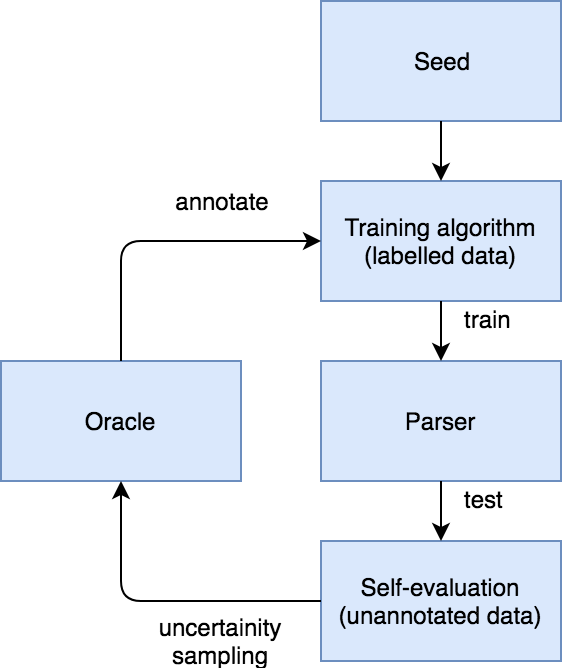
\includegraphics[width=0.6\linewidth]{flowchart}
	\caption{Active Learning Dependency Parsing model: Seed data is used to initialise the training. Subsequently, the model selects unannotated examples and sends it to the oracle which sends it the annotated trees. The labelled data is merged with these new examples and this is used to retrain the parser.}
	\label{fig:flowchart}
\end{figure}

Active learning is a special case of semi-supervised learning in which the learning algorithm is able to interactively query the user (oracle) and obtain more information about the desired unlabelled examples\footnote{Active Learning Wiki \url{https://en.wikipedia.org/wiki/Active_learning_(machine_learning)}.}. This puts the burden of data collection on the learning system. The training algorithm is responsible for deciding which unannotated examples it will learn most from. It selects these examples from the set of unannotated data points and passes it to the oracle which provides the correct label for them. The algorithm then uses this new set of labelled data to retrain the model. Based on what it learns, the system repeatedly selects small batches of unlabelled data to get it labelled by the oracle. The process ends when the desired amount accuracy is attained or some limit is reached.

In this assignment we design an Active Learning Dependency Parser (see Fig. \ref{fig:flowchart}) that selects samples to be annotated using uncertainty sampling. The probabilistic parser assigns a probability to each sentence it parses, based on this it samples the examples it is most uncertain about. These examples are annotated and fed back to the system. The hope is that these examples will help the system learn the most amount of information about the underlying distribution.

\section{Model and Dataset}

We build our parser over the dependency parser developed by Chen et al. 2014. They implement a neural shift-reduce parser that decides the parser actions by picking the transition with the maximum final layer output. We convert this into a well defined probability by adding a softmax layer to the final layer. The total (raw) probability $P_{raw}(S)$ of a sentence $S$ of length $n$ is given by:

\begin{equation}
P_{raw}(S) = \prod_{i = 1}^{2n} {T}_i
\end{equation}

Here $T_i$ denotes the probability of the most probable parser action (shift or reduce) at step $i$. We also define a margin parse probability $P_{margin}(S)$ for each sentence as given by:

\begin{equation}
P_{margin}(S) = \prod_{i = 1}^{2n} \big(T_i^1 - T_i^2\big)
\end{equation}

Here $T_i^1$ denotes the probability of the most probable parser actions and $T_i^2$ denotes the same for the second most probable parser action in step $i$. Since each word in the sentence has to be moved once from the buffer onto the stack and then reduced once to assign a parent in the parse tree, the number of parser actions performed for a sentence is $2n$. We used 4 uncertainty sampling techniques to sample sentences from the unlabelled set -- random, length, raw parse probability (eq. 1) and margin parse probability (eq. 2). The first 2 serve as the baseline for our system. Since the length $n$ can vary from sentence to sentence the $P_{raw}(S)$ and $P_{margin}(S)$ are normalised by taking the $2n^{th}$ root.

We use the WSJ data from the Penn treebank for our experiments. Since, the entire treebank is too large we only use a portion of it for simulating out experiments. We divide the dataset into seed, training and test set. The seed set contains $50$ sentences and forms our initial labelled set. The training set contains $\sim4500$ sentences and the test set contains $\sim2000$ sentences.

\section{Implementation}
 
 We build \code{ActiveLearningDependencyParser} class as a wrapper over the \code{DependencyParser} class written by Chen et al. In each epoch, the parser is trained on the labelled dataset for \code{maxIter} number of iterations. This model is used to then sample new unannotated examples from the unlabelled set based on the \code{oraclePolicy}. We restrict the max number of sentences that are added in each epoch based on the number of total words (\code{maxNewLabels}). In our implementation this value is set 1500 but is configurable. Since, \code{DependencyParser} class only accepts training data that is written to disk, we create a \code{tmp/} in the runtime directory. This directory stores the \code{labelled.connlx} and \code{unlabelled.connlx} files. In each iteration we transfer some sentences from the unlabelled set to the labelled set based on the \code{oraclePolicy}. Due to this the majority of the computation time is spent doing disk I/O. For evaluating the different sampling policies, we keep track of the Label Attachment Score (LAS) on the test set after each epoch.
 
 \section{Experiments}
 
 We perform 2 main experiments that have been discussed in the following subsections:
 
 \begin{figure*}[htbp]
	\centering
	\captionsetup{justification=centering}
	\begin{subfigure}[b]{0.48\textwidth}
		\centering
		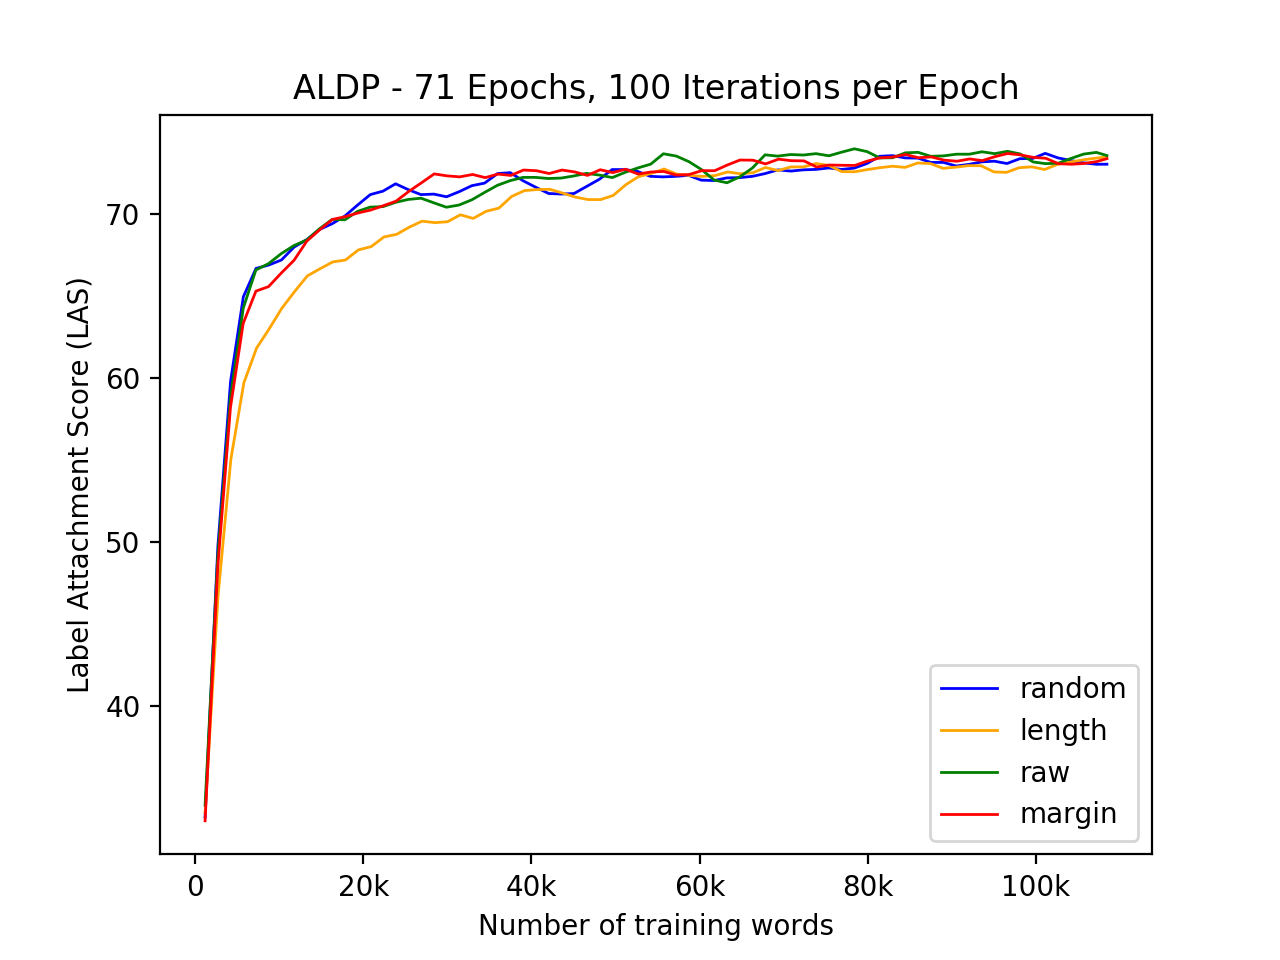
\includegraphics[width=\linewidth]{aldp_71_100_smooth}
		\caption{Full Test}
		\label{a}
	\end{subfigure}
	\centering
	\begin{subfigure}[b]{0.48\textwidth}
		\centering
		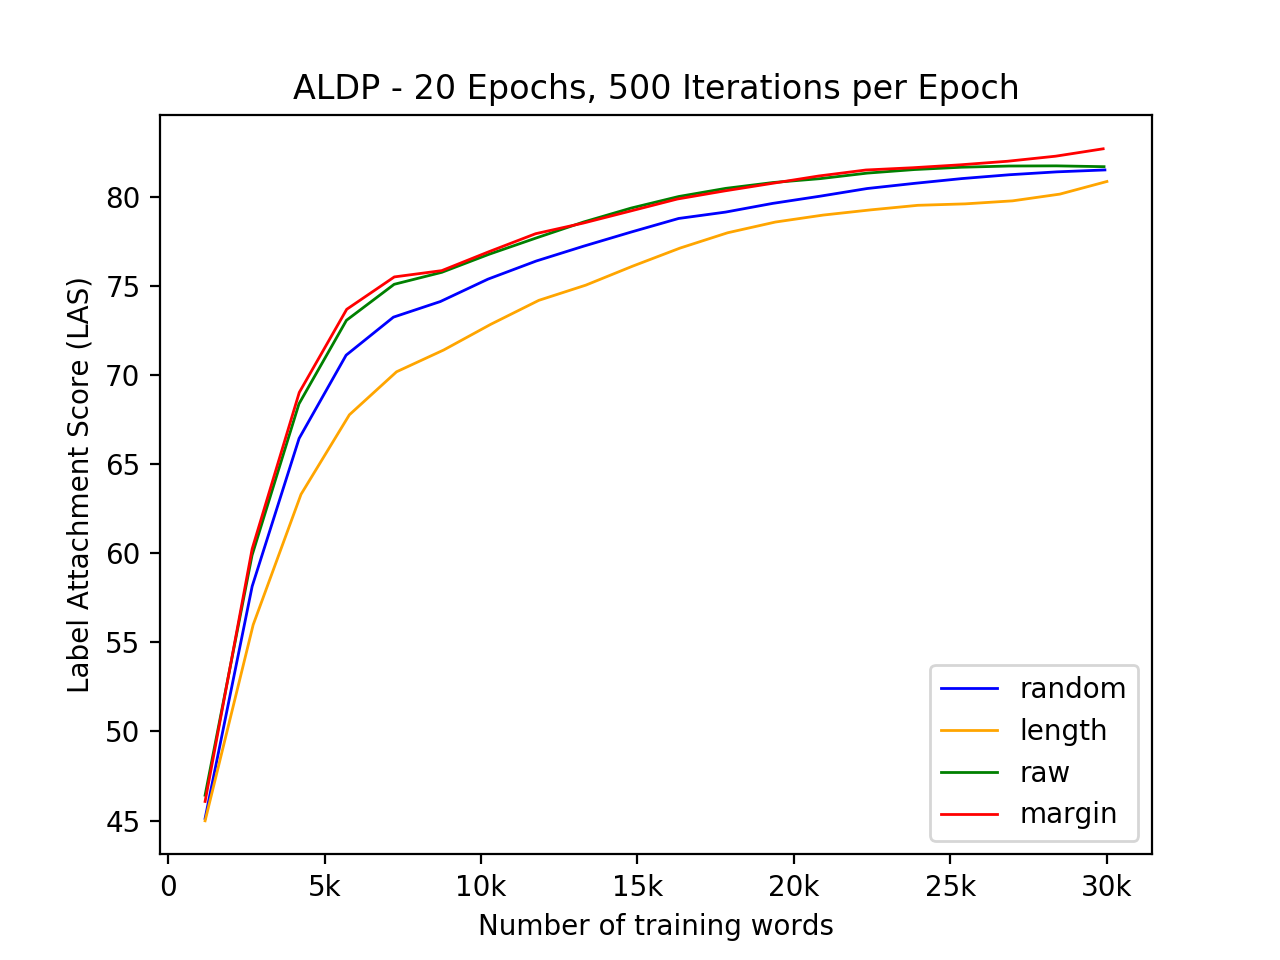
\includegraphics[width=\linewidth]{aldp_20_500_smooth}
		\caption{Partial Test}
		\label{b}
	\end{subfigure}
	\caption{Plot of LAS score vs number of training words for the experiments conducted. The LAS scores are evaluated on the test set after each epoch. The LAS score values are smoothed using the Savitzksy-Golay filter with a degree 3 polynomial and a window size 9.}
	\label{fig:graphs}
\end{figure*}
 
 \subsection{Experiment 1: Full Test}
 In this experiment we run the active learning epochs till all the sentences from the unlabelled sets are moved to the labelled set. Since each epoch takes a long time to run in the HTCondor cluster we reduced the \code{maxIter} value to 100. The full training takes 71 epochs to finish. The results of the experiment are presented in Fig. \ref{a}. We noticed that our random baseline policy (blue) was outperforming other more sophisticated sampling techniques like margin and raw. This lead us to believe that our model was not converging hence we devised the second experiment.
 
 \subsection{Experiment 2: Partial Test}
 Based on the previous experiment, we increase the number of iterations per epoch (\code{maxIter}) to 500. In order for the training process to terminate in a reasonable amount of time we restrict the number of active learning epochs to 20. Since, we are restricting the \code{maxNewLabels} to 1500 words, in 20 epochs the system is only able to incorporate $\sim30k$ words in the labelled set. The results of the experiment are displayed in Fig. \ref{b}. As expected the overall LAS score in experiment 2 are visibly higher than those of experiment 1.
 
\section{Discussion}
The following sections discusses some findings of our experiments.
 
\subsection{Uncertainty Sampling Methods vs Random Sampling}
If we look at the plot in Fig. \ref{b}, we can see that uncertainty sampling based on the raw and margin probabilities perform much better than the random sampling. This was expected because in random selection the system might select sentences that the parser already knows how to parse properly. So the system doesn't learn anything new with those training examples. Using raw and margin probabilities on the other hand allow the parser to choose sentences that the parser is most uncertain about. Hence, providing the accurate labels for these examples allow the parser to glean the most amount of information about the underlying distribution. On the other hand we notice that random sampling outperforms length based sampling. This was not expected. The most likely reason for this is that English language recursive in nature. Dependency parsers are able to learn this recursive nature fairly early on. The longer sentences are long because they have multiple recursive phrases. The parser already know how to parse these properly. Instead, dependency parses face difficulties parsing garden-path sentences. Random sampling allows the system to get the true annotations of a few of such sentences hence, it outperforms length-based sampling. We do not see the same trends in Fig. \ref{a}, this is most likely because the models are underfitting due to less number of iterations per epoch.

\subsection{Comparison Between Raw and Margin Probability Based Sampling}
As we can see from Fig. \ref{b}, margin probability based uncertainty sampling performs the best out of all 3, followed closely by the raw probability based uncertainty sampling. Both these sampling techniques outperform random and length based sampling by a noticeable margin. This was expected since probability based sampling allows the parser to choose examples from which it can learn the most. However, we expected margin based sampling to outperform raw based sampling by a larger margin. In some scenarios, the difference between the probabilities of the top 2 choices reveal more information about the uncertainty of choices than the absolute probability of the top choice. If the difference between the top 2 choice is large we have more confidence on the parser action. Based on the results it looks like that the margin probabilities does help the active learning system but for most sentences the difference between the top 2 choices is not that low hence, the probability values are almost similar to the raw probabilities.

\subsection{Effect of Active Learning on the Learning Curve}
If we looks at the plot from Fig. \ref{a}, we can see that the different uncertainty sampling do not affect the learning uniformly across epochs. The LAS score different between the various methods is more pronounced in the initial stages of the training. This was expected because active learning only helps during the initial stages of training. Once the model has enough number of representative examples of the sentences it does not need sampling policies to choose further examples. We see that once the number of labelled training words reaches $\sim60k$ the learning curve almost flattens. However, the differences between the different oracle policies are quite noticeable before that.

\subsection{Comparison with Hwa et al. paper}
In our approach, random policy takes $\sim11700$ words to attain an LAS score of 75. On the other hand margin and raw policies take $\sim8700$ words to attain the same LAS score, which is 25.6\% less than the number of samples for random. Hwa et al. obtain a 36\% reduction in the number of brackets. This is most likely because we are using the state-of-the-art neural dependency parser from Stanford. So the random baseline is harder to beat. Another difference is that Hwa et al. use entropy to sample unannotated data while in our case we use the probability values to do this.

\section{Conclusion}
Our results reinforce the claim that active learning can be used to increase the data efficiency of the Stanford neural dependency parser. With increase in the manually annotated data, the performance in both the experiments increases. Also we see that uncertainty sampling based on margin probability score outperforms other sampling techniques.

\end{document}
